\documentclass{article} % For LaTeX2e
\usepackage{nips14submit_e,times}
\usepackage{amsmath}
\usepackage{amsthm}
\usepackage{amssymb}
\usepackage{mathtools}
\usepackage{hyperref}
\usepackage{url}
\usepackage{algorithm}
\usepackage[noend]{algpseudocode}
%\documentstyle[nips14submit_09,times,art10]{article} % For LaTeX 2.09

\usepackage{graphicx}
\usepackage{caption}
\usepackage{subcaption}

\def\eQb#1\eQe{\begin{eqnarray*}#1\end{eqnarray*}}
\def\eQnb#1\eQne{\begin{eqnarray}#1\end{eqnarray}}
\providecommand{\e}[1]{\ensuremath{\times 10^{#1}}}
\providecommand{\pb}[0]{\pagebreak}
\DeclarePairedDelimiter\ceil{\lceil}{\rceil}
\DeclarePairedDelimiter\floor{\lfloor}{\rfloor}

\newcommand{\E}{\mathrm{E}}
\newcommand{\Var}{\mathrm{Var}}
\newcommand{\Cov}{\mathrm{Cov}}

\def\Qb#1\Qe{\begin{question}#1\end{question}}
\def\Sb#1\Se{\begin{solution}#1\end{solution}}

\newenvironment{claim}[1]{\par\noindent\underline{Claim:}\space#1}{}
\newtheoremstyle{quest}{\topsep}{\topsep}{}{}{\bfseries}{}{ }{\thmname{#1}\thmnote{ #3}.}
\theoremstyle{quest}
\newtheorem*{definition}{Definition}
\newtheorem*{theorem}{Theorem}
\newtheorem*{lemma}{Lemma}
\newtheorem*{question}{Question}
\newtheorem*{preposition}{Preposition}
\newtheorem*{exercise}{Exercise}
\newtheorem*{challengeproblem}{Challenge Problem}
\newtheorem*{solution}{Solution}
\newtheorem*{remark}{Remark}
\usepackage{verbatimbox}
\usepackage{listings}
\usepackage{mathrsfs}
\title{Functional Analysis: \\
Problem Set III}


\author{
Youngduck Choi \\
CIMS \\
New York University\\
\texttt{yc1104@nyu.edu} \\
}


% The \author macro works with any number of authors. There are two commands
% used to separate the names and addresses of multiple authors: \And and \AND.
%
% Using \And between authors leaves it to \LaTeX{} to determine where to break
% the lines. Using \AND forces a linebreak at that point. So, if \LaTeX{}
% puts 3 of 4 authors names on the first line, and the last on the second
% line, try using \AND instead of \And before the third author name.

\newcommand{\fix}{\marginpar{FIX}}
\newcommand{\new}{\marginpar{NEW}}

\nipsfinalcopy % Uncomment for camera-ready version

\begin{document}


\maketitle

\begin{abstract}
This work contains solutions to the exercises of the problem set III.
\end{abstract}

\bigskip

\begin{question}[1]
\hfill
\begin{figure}[h!]
  \centering
    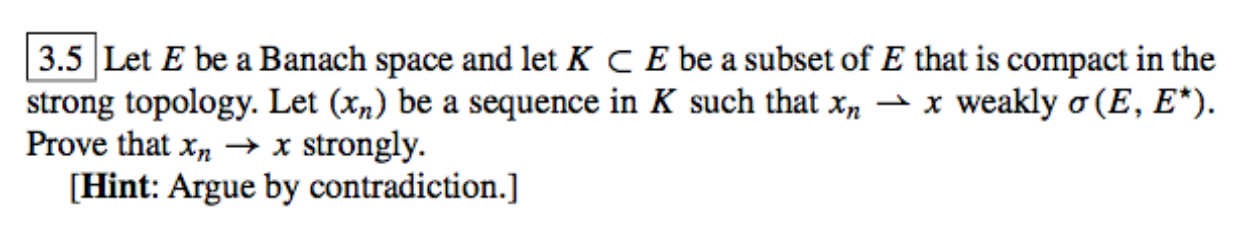
\includegraphics[width=0.7\textwidth]{funcA-h-e3-p1.png}
\end{figure}
\end{question}
\begin{solution} \hfill \\
Suppose $x_n \not\to x$ strongly. Then, there exists $\epsilon > 0$ and $\{x_{n_k}\}$
such that 
\eQnb
|x_{n_k} - x| > \epsilon \label{eq:1.1}
\eQne
for all $k \geq 1$. By the compactness of $K$ in strong topology, there exists
a further subsequence $\{x_{n_{k_l}}\}$ such that
\eQb
\lim_{l \to \infty} x_{n_{k_l}} = y
\eQe
for some $y \in K$. From ~\eqref{eq:1.1}, $y \neq x$. Now, since convergence
in strong topology implies convergence in weak topology, we have
\eQb
x_{n_{k_l}} \to_{\text{weak}} y \>\>\> &\text{as}& \>\>\> l \to \infty.
\eQe  
From our assumption, however, $x_{n} \to_{\text{weak}} x$ as $n \to \infty$,
so by Hausdroff property of weak topology
$x_{n_{k_l}} \to_{\text{weak}} x$ as $l \to \infty$.
This contradicts the uniquness of limit property of weak topology, which also
arises from Hausdorff property of weak topology. We have a contradiction, and
we are done.

\hfill  \qed

\end{solution}

\newpage

\begin{question}[2]
\hfill
\begin{figure}[h!]
  \centering
    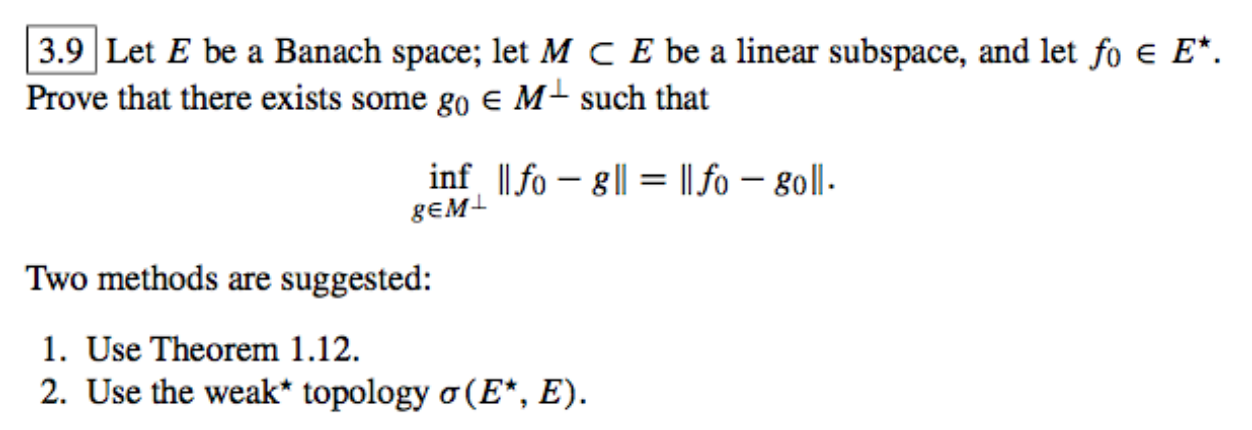
\includegraphics[width=0.7\textwidth]{funcA-h-e3-p2.png}
\end{figure}
\end{question}
\begin{solution} \hfill \\
By Banach-Alaoglu, $B_{E^*}$ is weak-* compact, and we claim that $M^{\perp}$ is
closed in weak-*, because $M^{\perp}$ is closed in strong topology in $E^*$. 
Let $f \in E^*$ such that there exists $\{f_n\} \subset M^{\perp}$ with 
$f_n to f$ strongly. Then,
\eQb
\lim_{n \to \infty} <f_n,x> = <f,x>. 
\eQe 


\end{solution}

\newpage

\begin{question}[3]
\hfill
\begin{figure}[h!]
  \centering
    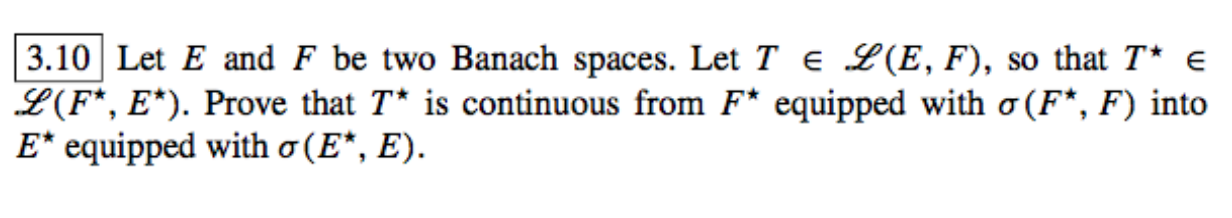
\includegraphics[width=0.7\textwidth]{funcA-h-e3-p3.png}
\end{figure}
\end{question}
\begin{solution} \hfill \\
\end{solution}

\newpage

\begin{question}[4]
\hfill
\begin{figure}[h!]
  \centering
    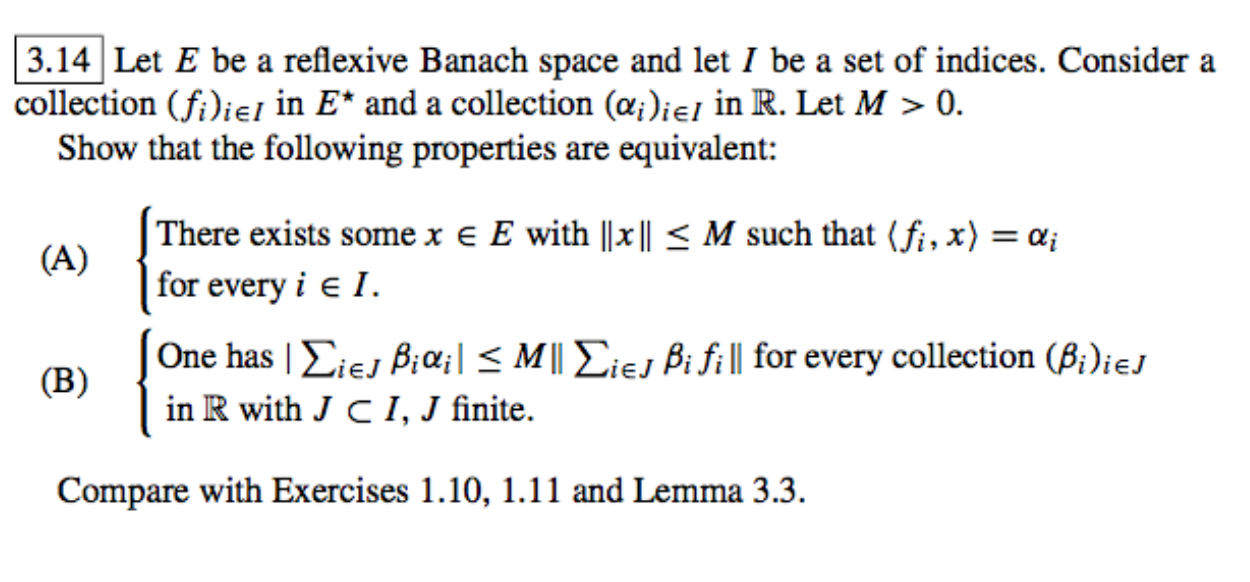
\includegraphics[width=0.7\textwidth]{funcA-h-e3-p4.png}
\end{figure}
\end{question}
\begin{solution} \hfill \\
$(A) \implies (B)$ is obvious. For a moment, we assume the result of exercise 1.10
in Brezis.
Suppose (B) is true. Then, by 1.10, there exists $\phi_0 \in E^{**}$ such that 
\eQb
||f|| \leq M \>\>\> &\text{and}& \>\>\> <\phi_0,f_i> = \alpha_i
\eQe
for all $i \in I$. Then, by reflexivity of $E$, there exists $x_0 \in E$ such that
\eQb
||x_0|| \leq M  \>\>\> &\text{and}& \>\>\> <f,x_0> = \alpha_i 
\eQe
for all $i \in I$. Hence, it suffices to prove the result of 1.10. In particular,
we need $(B) \implies (A)$ direction. Let $G$ be the vector space spanned by
$\{x_i\}_{i \in I}$. Define $g:G \to \mathbb{R}$ by
\eQb
g(x) &=& \sum_{i \in J} \beta_i \alpha_i 
\eQe
where $x = \sum_{i \in J} \beta_i x_i$. $g$ is well-defined and bounded by assumption
(B). Now, extend $g$ to the whole of $E$ by corollary of 

\end{solution}

\newpage

\begin{question}[5]
\hfill
\begin{figure}[h!]
  \centering
    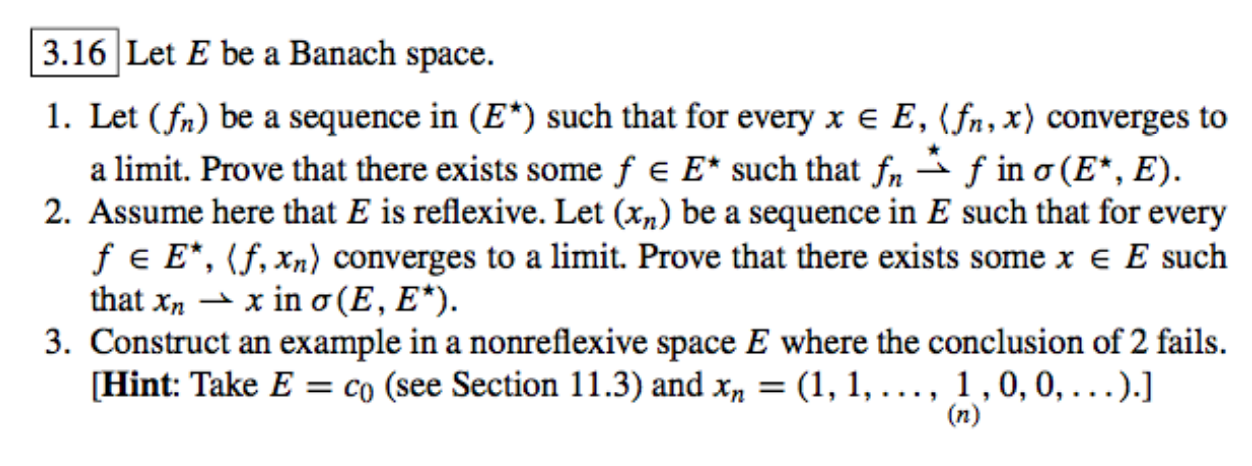
\includegraphics[width=0.7\textwidth]{funcA-h-e3-p5.png}
\end{figure}
\end{question}
\begin{solution} \hfill \\
Let $f:E \to \mathbb{R}$ be defined by
\eQb
<f,x> &=& \lim_{n \to \infty} <f_n,x> \>\>\> (x \in E).
\eQe
Then, $f$ is linear, because by linearty of $\{f_n\}$,
\eQb
<f,x+y> &=& \lim_{n \to \infty} <f_n,x+y> = \lim_{n \to \infty} <f_n,x> + <f_n,y> \\
&=& \lim_{n \to \infty} <f_n,x> + \lim_{n \to \infty} <f_n,y> = <f,x> + <f,y>
\eQe
for any $x,y \in E$ and
\eQb
<f,\lambda x> &=& \lim_{n \to \infty} <f_n,\lambda x> = \lambda \lim_{n \to \infty}
<f,x> 
\eQe
for any $\lambda \in \mathbb{R}$ and $x \in E$. If we show that $f$ is bounded,
or continuous then we are done, since
\eQb
f_n \to f \>\>\> \text{in weak-*} &\iff& <f_n,x> \to <f,x> \text{as}
\eQe 
\end{solution}

\newpage

\begin{question}[6]
\hfill
\begin{figure}[h!]
  \centering
    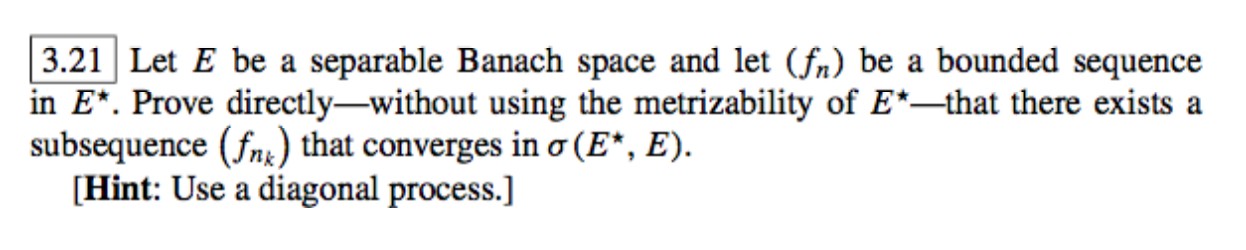
\includegraphics[width=0.7\textwidth]{funcA-h-e3-p6.png}
\end{figure}
\end{question}
\begin{solution} \hfill \\
As $E$ is separable, there exists $\{a_i\}$, 
a dense countable subset of $E$. 
Since $\{f_n\}$ are bounded in $E^*$, $\{<f_{n}, a_1> \}$ is bounded in $\mathbb{R}$.
Hence, we can choose a subsequence $\{n_k\}$, with relabeling $\{(1,k)\}$ such that 
\eQb
\lim_{k \to \infty} <f_{1,k},a_1> \>\>\> \text{exists}.
\eQe
Now, with the fact that $\{<f_{n},a_2 > \}$ is bounded in $\mathbb{R}$,
choose a further subsequence $\{n_{k_l}\}$ from $\{n_k\}$, with relabeling
$\{(2,k)\}$ such that
\eQb
\lim_{k \to \infty} <f_{2,k},a_2> \>\>\> \text{exists}.
\eQe
Repeat this process inductively, so that we have chosen $f_{l,k}$ for all $l,k \in
\mathbb{N}$. Then, consider $\{ g_{l} \} = \{f_{l,l}\}$, 
which is the standard diagonal sequence. 
Then, by choice
\eQb
\lim_{l \to \infty} <g_l, a_i> \>\>\> \text{exists}
\eQe 
for any $i \in \mathbb{N}$. Let $g:E \to \mathbb{R}$ such that
\eQb
<g , a_i> &=& \lim_{l \to \infty} <g_l, a_i>
\eQe 
for all $i \in \mathbb{N}$, and for any $x \in E \setminus \{a_i\}$, 
by density of $\{a_i\}$,
choose $\{a_p\} \subset \{a_i \}$ such that $\lim_{p \to \infty} a_p = x$ and 
\eQb
<g,x> &=& \lim_{p \to \infty} <g, a_p>. 
\eQe
This is well-defined, and $g \in E^*$. By definition,
 

\end{solution}



\end{document}
